The name of the second prototype, which has been developed in Valencia, is Tritium-IFIC 1 that is shown in the figure \ref{fig:Tritium_IFIC_1}. This prototype has a internal volume of $0.118~\liter$ and 64 scintillating fibers read out by the same PMT that in the previous prototype. 

In this prototype, the problems found in the first prototype was solved. As we cannot change the quality of the fiber surface we will try to mitigate their effect.

\begin{figure}[htbp]
\centering
\subfigure[Protoype of Tritium-IFIC 1\label{fig:TritiumIFIC1prototype}]
{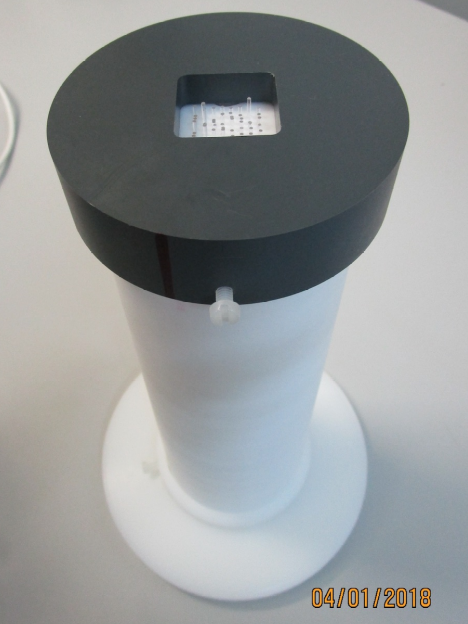
\includegraphics[width=40mm]{./Figuras/Prototype_Tritium_1.png}}\hspace{10mm}
\subfigure[Hole matrix \label{fig:FiberArrangement1}]
{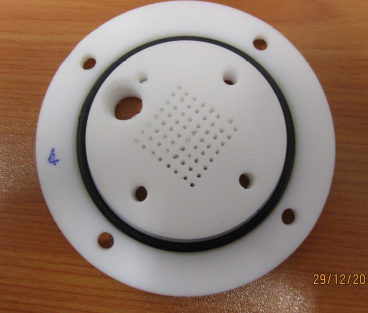
\includegraphics[width=50mm]{./Figuras/Arrange_fibers_piece.png}}\hspace{10mm}
\subfigure[Fiber arrangement matrix \label{fig:FiberArrangement2}]
{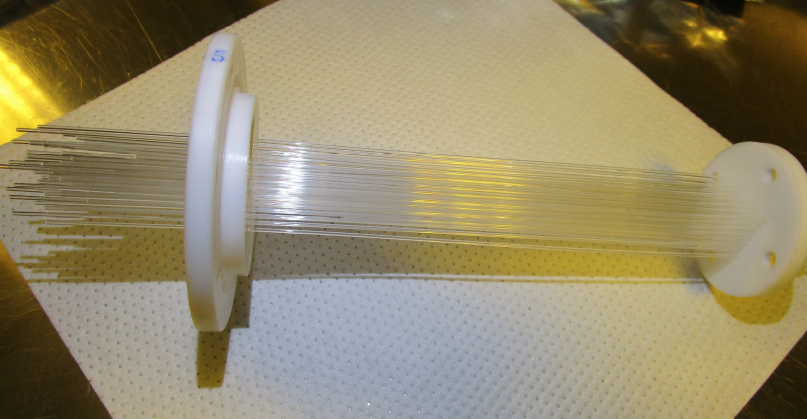
\includegraphics[width=100mm]{./Figuras/Arrange_fibers.png}}
\caption{Tritium-IFIC 1 prototype.} \label{fig:Tritium_IFIC_1}
\end{figure}

First, as you can see in the figure \ref{fig:FiberArrangement2}, the fibers of this detector will be arranged straight, that is, without any curve. With this change we got minimize the amount of photons which escape from the fibers.

Second, we arrange the fibers in a equidistant distance between them. We achieved it with several internal hole matrix as you can see in the figure \ref{fig:FiberArrangement1}. The final aspect of this arranged is shown in the figure \ref{fig:FiberArrangement2}. With this structure we ensure that the active volume of our detector is the one which we know and, with it, we can obtain our correct specific efficiency.

On top of that, we have done some modifications with which we hope to improve the efficiency of our detector.

On the one hand, a special fiber cleaning process has been included consisting of several baths with a neutral soap, pure water and isopropanol inside an ultrasound machine, all this process inside a clean room. With this process we get better wetting properties for fibers and, by extension, we will increase the capacity of this prototype for the detection of tritium.

This process were checked in order to be sure that it don't affect to the light production and collection of the fibers, whose result is shown in the figure \ref{fig:CleaningProcess}.

\begin{figure}[htbp]
\centering
\subfigure[Measurement of the light produced in a bunch of $25$ fibers of $20~\cm$ due to the \ce{^{90}Sr} source \label{fig:SrCleaning}]{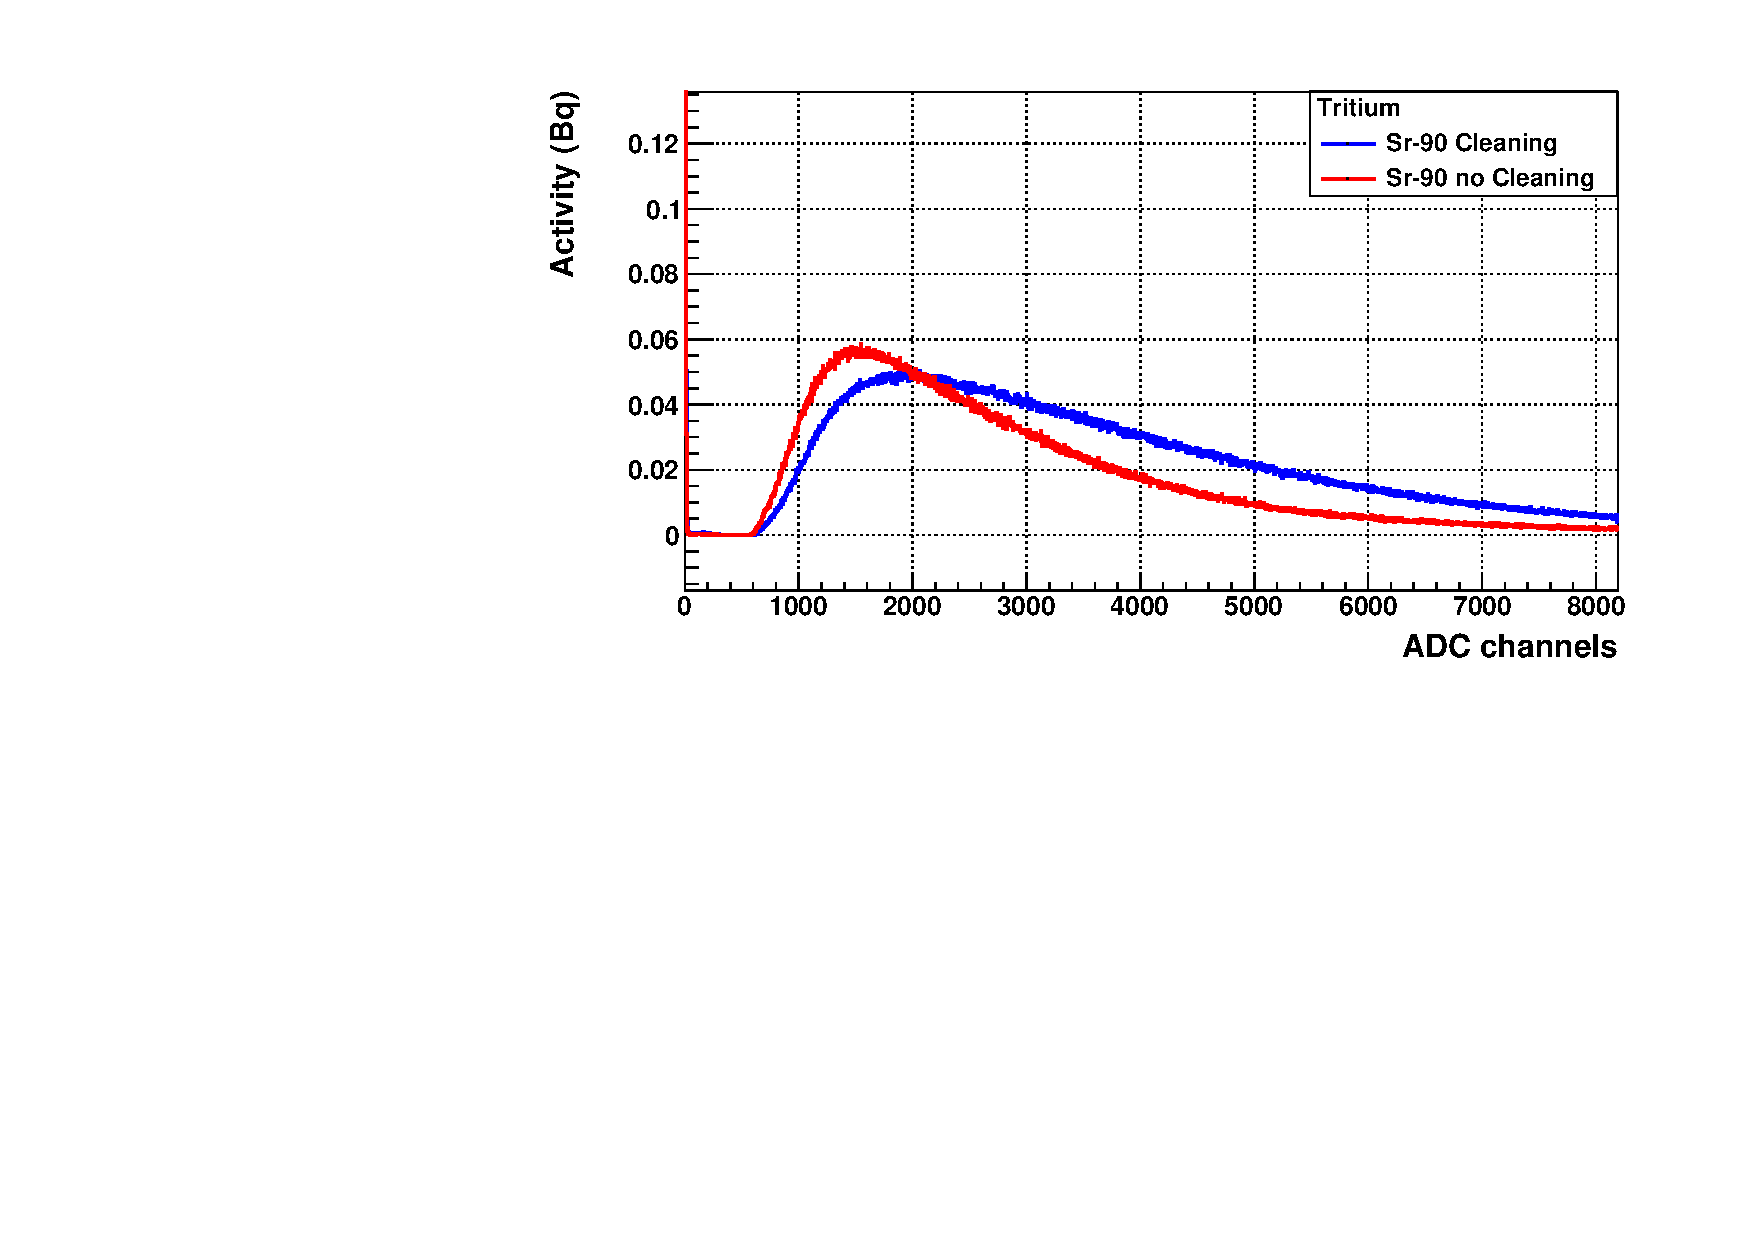
\includegraphics[width=72mm]{./Figuras/Sr_90s.pdf}}\hspace{10mm}
\subfigure[Measurement of the light produced in a bunch of $25$ fibers of $20~\cm$ due to the \ce{^{137}Cs} source \label{fig:CoCleaning}]{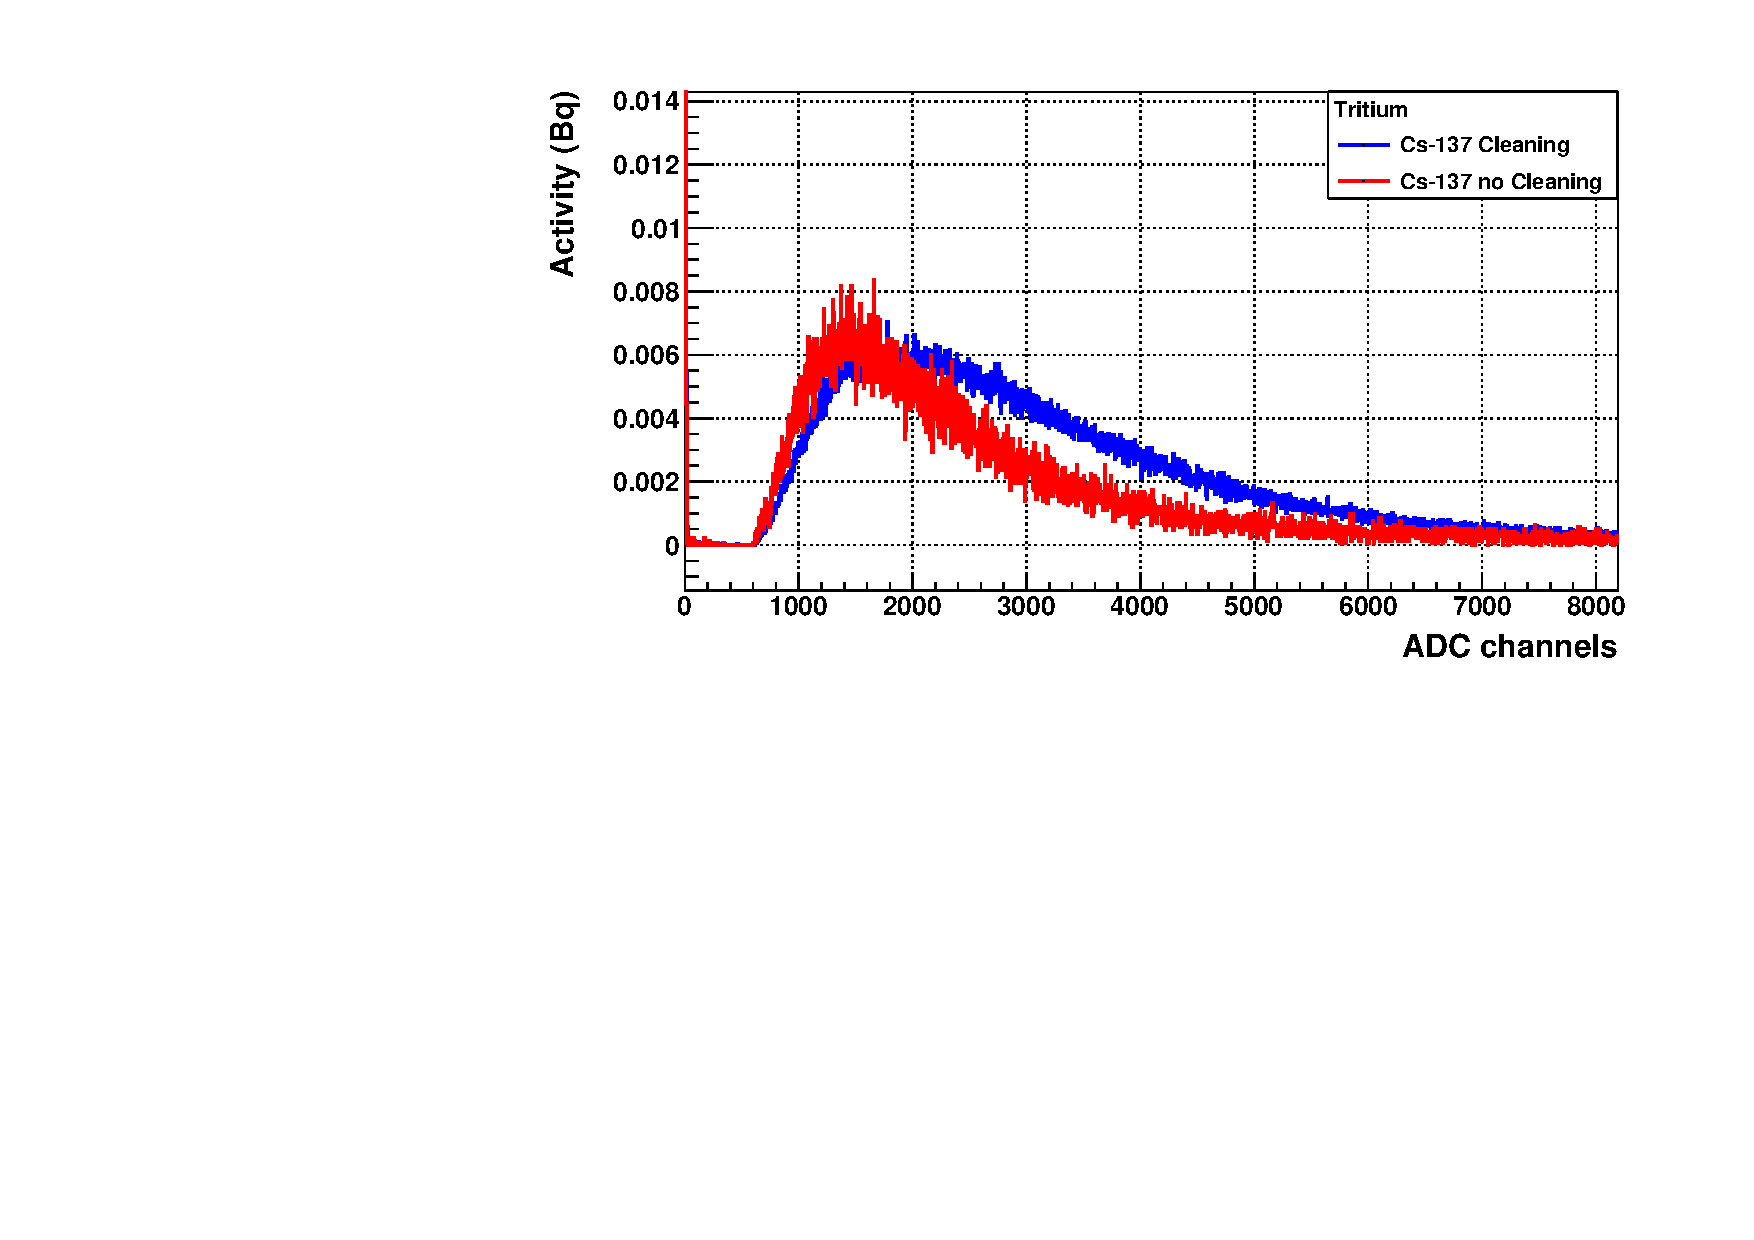
\includegraphics[width=72mm]{./Figuras/Cs_137s.pdf}}
\caption{Cuantification of the improvement of polishing process} \label{fig:CleaningProcess}
\end{figure}

Here we can see that not only it doesn't get worse the light collection efficiency of the fibers but this process improve it. We can see that in both cases event numbers is quite similar but this events has higher energy.

On the other hand we have used teflon for the material of the vessel since its reflectivity is quite similar to 100\%. Therefore if any  photon escape from the fiber it can arrive to any wall of the vessel and come back to the fiber. It will increse the efficiency of our detector.

After we do all this modifications we did the same measurements for check the efficiency of this detector, that's is, one for getting the background signal of our system and another for the tritium signal whose activity was the same that the experience with the previous prototype, $53.385~\mega\becquerel/\liter$. 

We have to take into account that with this prototype we don't make coincidence because this prototype only can measure by one side of the fibers. It is not important because we still use the discriminator with which we remove the termical noise of the PMTs. Other events which we don't remove with this discriminator, like cosmic events with higher energy, it affect statistically equal to the background than the signal, thus, it don't affect to the tritium signal (difference)

The measurements which was done with  this prototype is shown in the figure \ref{fig:Tritium_IFIC_1_Signals}.

\begin{figure}[htbp]
\centering
\subfigure[Signal and Background of Tritium-IFIC 1 \label{fig:SignalsTritiumIFIC1}]{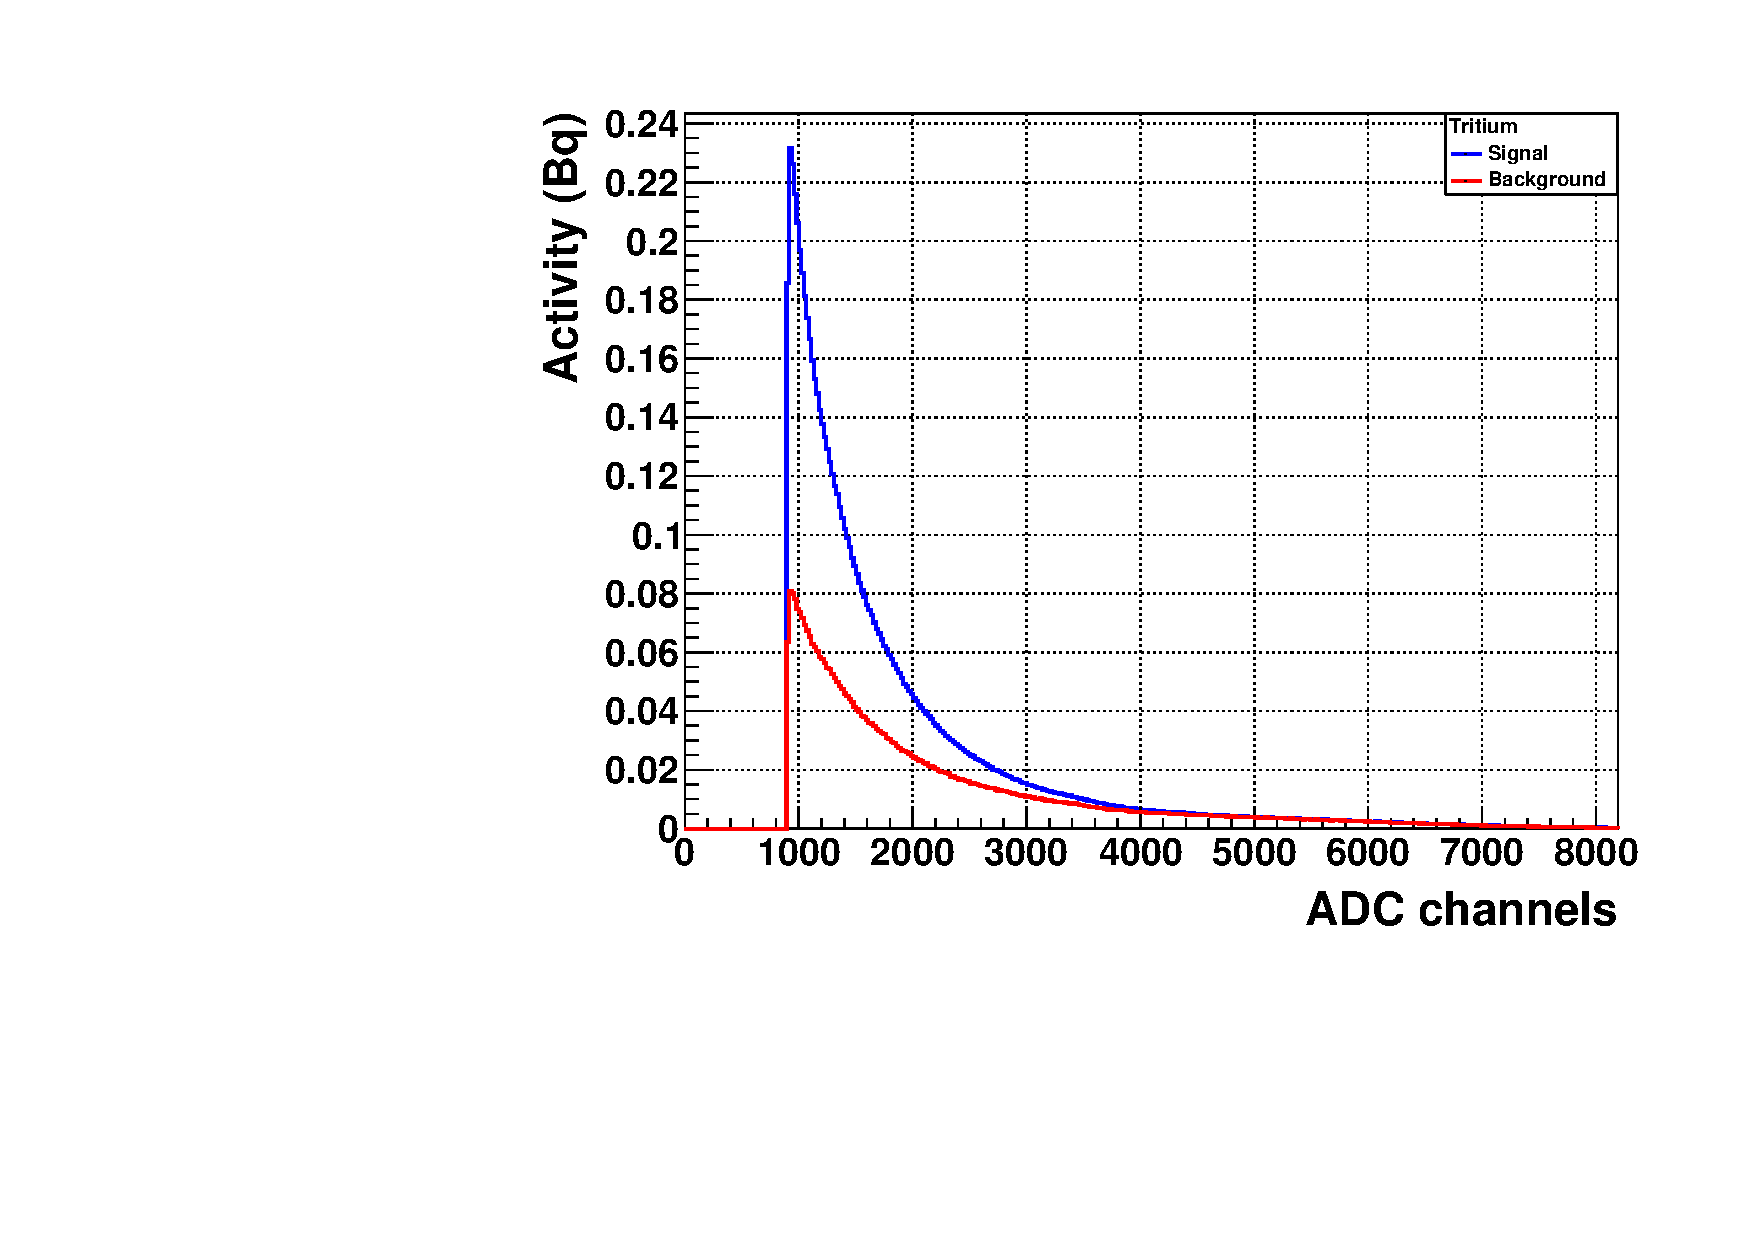
\includegraphics[width=70mm]{./Figuras/Signal_Background_Tritium1.pdf}}
\subfigure[Clear signal of tritium \label{fig:ClearSignalTritiumIFIC1}]{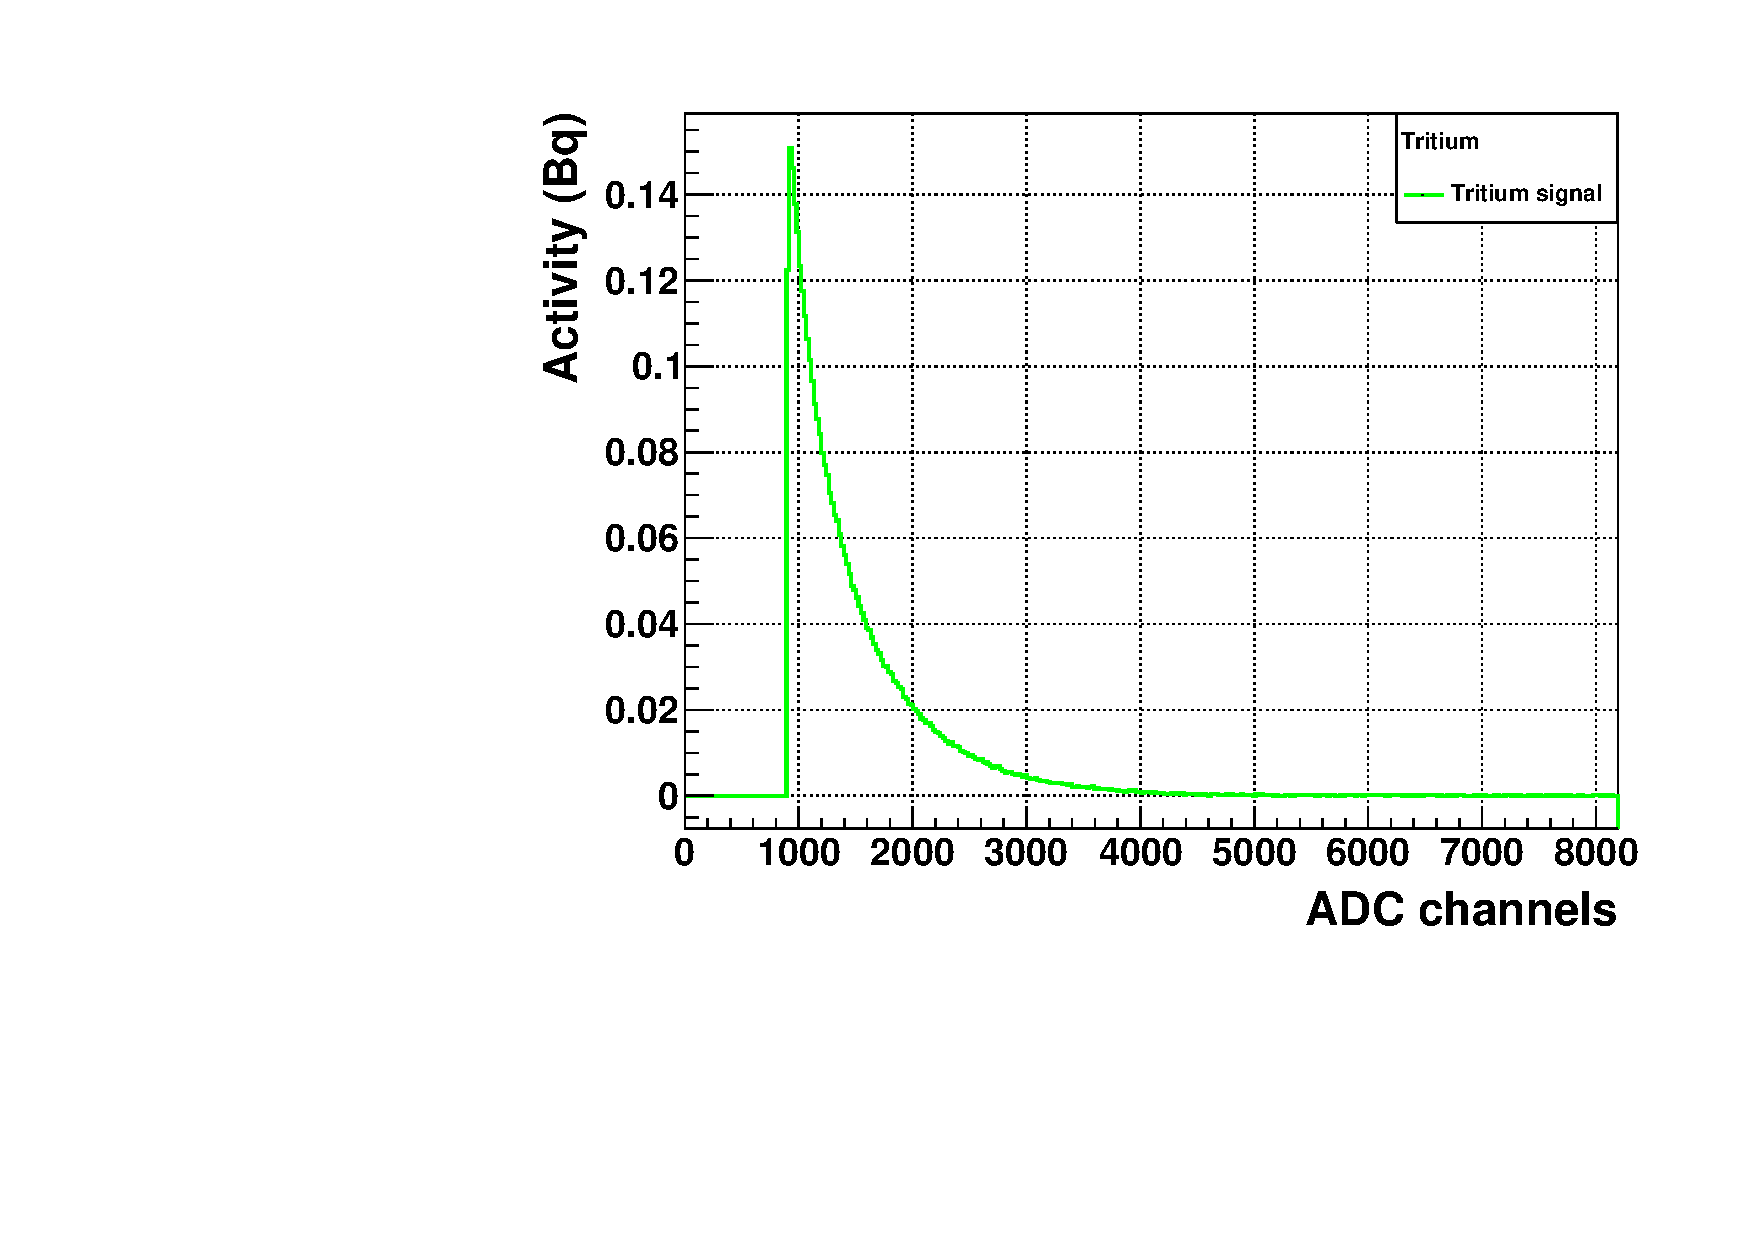
\includegraphics[width=70mm]{./Figuras/Signal_Tritium_Tritium1.pdf}}
\caption{Tritium signals of Tritium-IFIC 1 prototype.} \label{fig:Tritium_IFIC_1_Signals}
\end{figure}

We have obtained $4.17$ counts per second with this prototype and this tritium solution. It means that the efficiency of this prototype is $\varepsilon_{det} = 7.81 \cdot 10^{-5}~(\ce{counts}/\sec)/(\kilo\becquerel/\liter)$. Now the active surface is $A_{suf} = 402.124~\cm^2$ so the specific efficiency is $\varepsilon_{spe} = 1.94 \cdot 10^{-7}~(\ce{counts}/\sec)/(\cm^{2}\kilo\becquerel/\liter)$. 

We can see that our efficiency has improved in a ten factor. In any case it is one order smaller that the efficiency of other detectors with the same objective. It could be due to the pile-up of our system since we are working with higher tritium activities than the other experiments. We are working with activities of the order of $10^{7}~\becquerel/\liter$  and the other experiments was done with activities of the order of $10^{4}~\becquerel/\liter$. It could affect to our measurements in several ways like pile-up or producing a damage of the fibers, both effects contribute to reduce the efficiency of this prototype. It is something which we will check in a near future with prototypes fill with lesser activities of the tritium solution.

The only problem which we have found with this prototype is that we cannot read with two PMTs in coincidence. It is a problem because, although most of the PMT dark current does not overcome the discriminator level, we have to take into account that this discriminator level is very low  since the energy events of tritium are very small. Due to that, it is possible, but unlikely, that some dark current events of the PMT overcome it and contribuite to the signal of the detector. 